\documentclass[11pt,letterpaper]{article}

\addtolength{\oddsidemargin}{-.875in}
\addtolength{\evensidemargin}{-.875in}
\addtolength{\textwidth}{1.75in}

\addtolength{\topmargin}{-.875in}
\addtolength{\textheight}{1.75in}

\usepackage[utf8]{inputenc}
\usepackage{caption} % for table captions
\usepackage{amsmath} % for multi-line equations and piecewises
\DeclareMathOperator{\sign}{sign}
\usepackage{graphicx}
\usepackage{relsize}
\usepackage{xspace}
\usepackage{verbatim} % for block comments
\usepackage{subcaption} % for subfigures
\usepackage{enumitem} % for a) b) c) lists
\newcommand{\Cyclus}{\textsc{Cyclus}\xspace}%
\newcommand{\Cycamore}{\textsc{Cycamore}\xspace}%
\newcommand{\deploy}{\texttt{d3ploy}\xspace}%
\newcommand{\Deploy}{\texttt{D3ploy}\xspace}%
\usepackage{tabularx}
\usepackage{color}
\usepackage{multirow}
\usepackage{float} 
\usepackage[acronym,toc]{glossaries}
%\include{acros}
\definecolor{bg}{rgb}{0.95,0.95,0.95}
\newcolumntype{b}{X}
\newcolumntype{f}{>{\hsize=.15\hsize}X}
\newcolumntype{s}{>{\hsize=.5\hsize}X}
\newcolumntype{m}{>{\hsize=.75\hsize}X}
\newcolumntype{r}{>{\hsize=1.1\hsize}X}
\usepackage{titling}
\usepackage[hang,flushmargin]{footmisc}
\renewcommand*\footnoterule{}
\usepackage{tikz}

\usetikzlibrary{shapes.geometric,arrows}
\tikzstyle{process} = [rectangle, rounded corners, 
minimum width=1cm, minimum height=1cm,text centered, draw=black, 
fill=blue!30]
\tikzstyle{arrow} = [thick,->,>=stealth]

\graphicspath{}

\begin{document}

\section{2D-neutronics}

\subsection{2D-unitcell-reflec-actionB}

	\begin{itemize}
		\item Input file: \textit{2D-unitcell-reflec-actionB.i}
		\item Mesh: \textit{2D-unitcell-reflecB.msh}
		\item Transient problem.
	\end{itemize}

Figure \ref{fig:2D-unitcell-reflecB} displays the geometry.
Figures \ref{fig:2D-unitcell-reflecB1} and \ref{fig:2D-unitcell-reflecB2} show the results.

	\begin{figure}[htbp!]
		\centering
		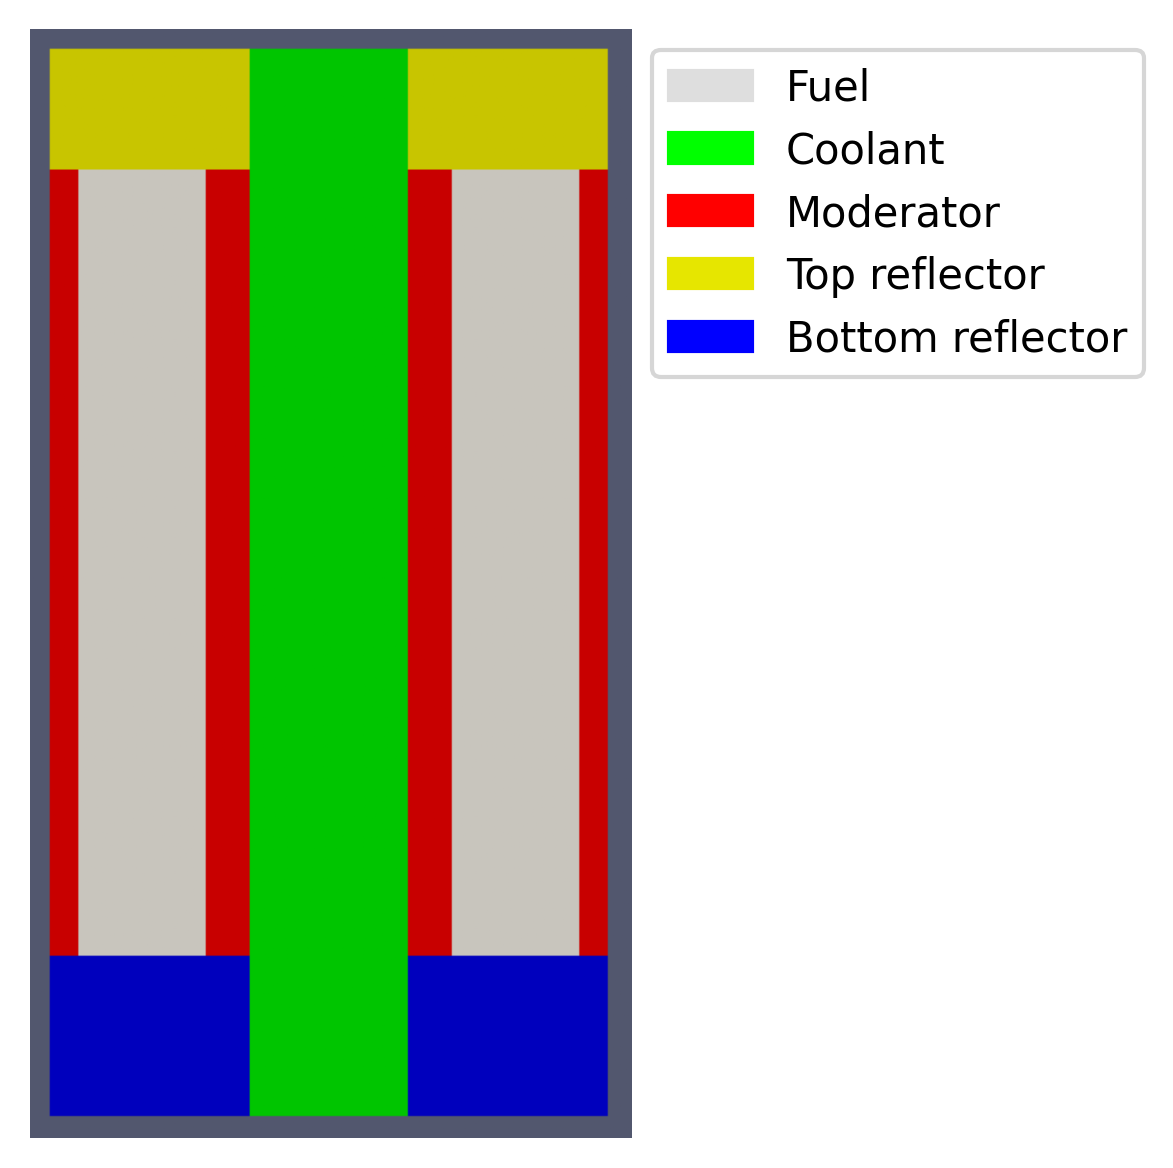
\includegraphics[height=5cm]{2D-unitcell-reflecB-mesh}
		\caption{\textit{2D-unitcell-reflecB} scaled down geometry.}
		\label{fig:2D-unitcell-reflecB}
	\end{figure}

	\begin{figure}[htbp!]
		\centering
		\begin{subfigure}[t]{0.4\textwidth}
			\centering
			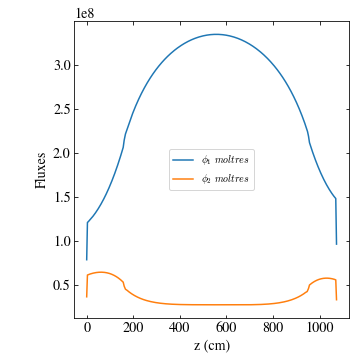
\includegraphics[width=\linewidth]{2D-unitcell-reflec-actionB1}
			\caption{Fuel centerline between points (0.94,-160,0) and (0.94,913,0).}
		\end{subfigure}
		\begin{subfigure}[t]{0.4\textwidth}
			\centering
			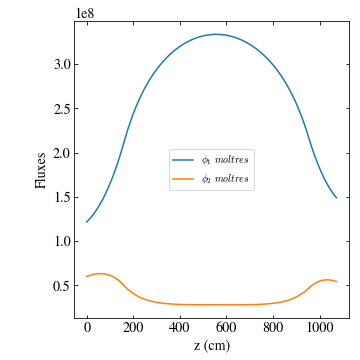
\includegraphics[width=\linewidth]{2D-unitcell-reflec-actionB2}
			\caption{Coolant centerline between points (2.82,-160,0) and (2.82,913,0).}
		\end{subfigure}
		\hfill
		\caption{Group 1 and 2 axial fluxes in different locations of the unitcell at 10 msec.}
		\label{fig:2D-unitcell-reflecB1}
	\end{figure}

	\begin{figure}[htbp!]
		\centering
		\begin{subfigure}[t]{0.4\textwidth}
			\centering
			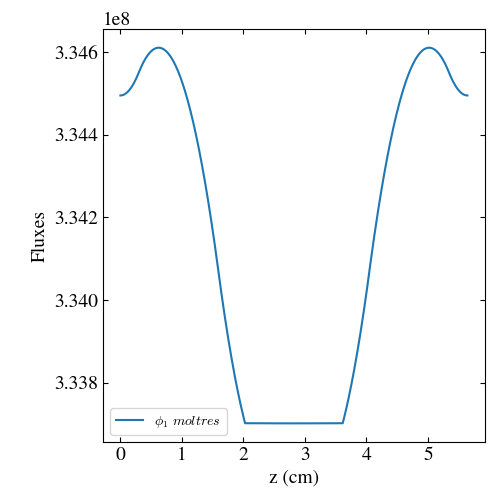
\includegraphics[width=\linewidth]{2D-unitcell-reflec-actionB3}
			\caption{Group 1.}
		\end{subfigure}
		\begin{subfigure}[t]{0.4\textwidth}
			\centering
			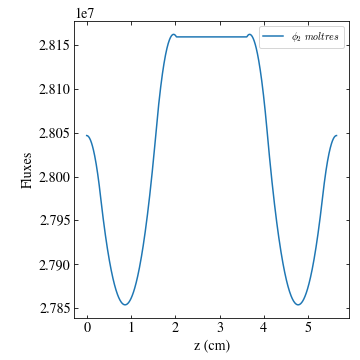
\includegraphics[width=\linewidth]{2D-unitcell-reflec-actionB4}
			\caption{Group 2.}
		\end{subfigure}
		\hfill
		\caption{Group 1 and 2 fluxes across the cell between points (0,400,0) and (5.64,400,0) at 10 msec.}
		\label{fig:2D-unitcell-reflecB2}
	\end{figure}

\subsection{2D-unitcell-reflec-action}

	\begin{itemize}
		\item Input file: \textit{2D-unitcell-reflec-action.i}
		\item Mesh: \textit{2D-unitcell-reflec.msh}
		\item Transient problem.
	\end{itemize}

Figure \ref{fig:2D-unitcell-reflec} displays the geometry.
Figures \ref{fig:2D-unitcell-reflec1} and \ref{fig:2D-unitcell-reflec2} show the results.

	\begin{figure}[htbp!]
		\centering
		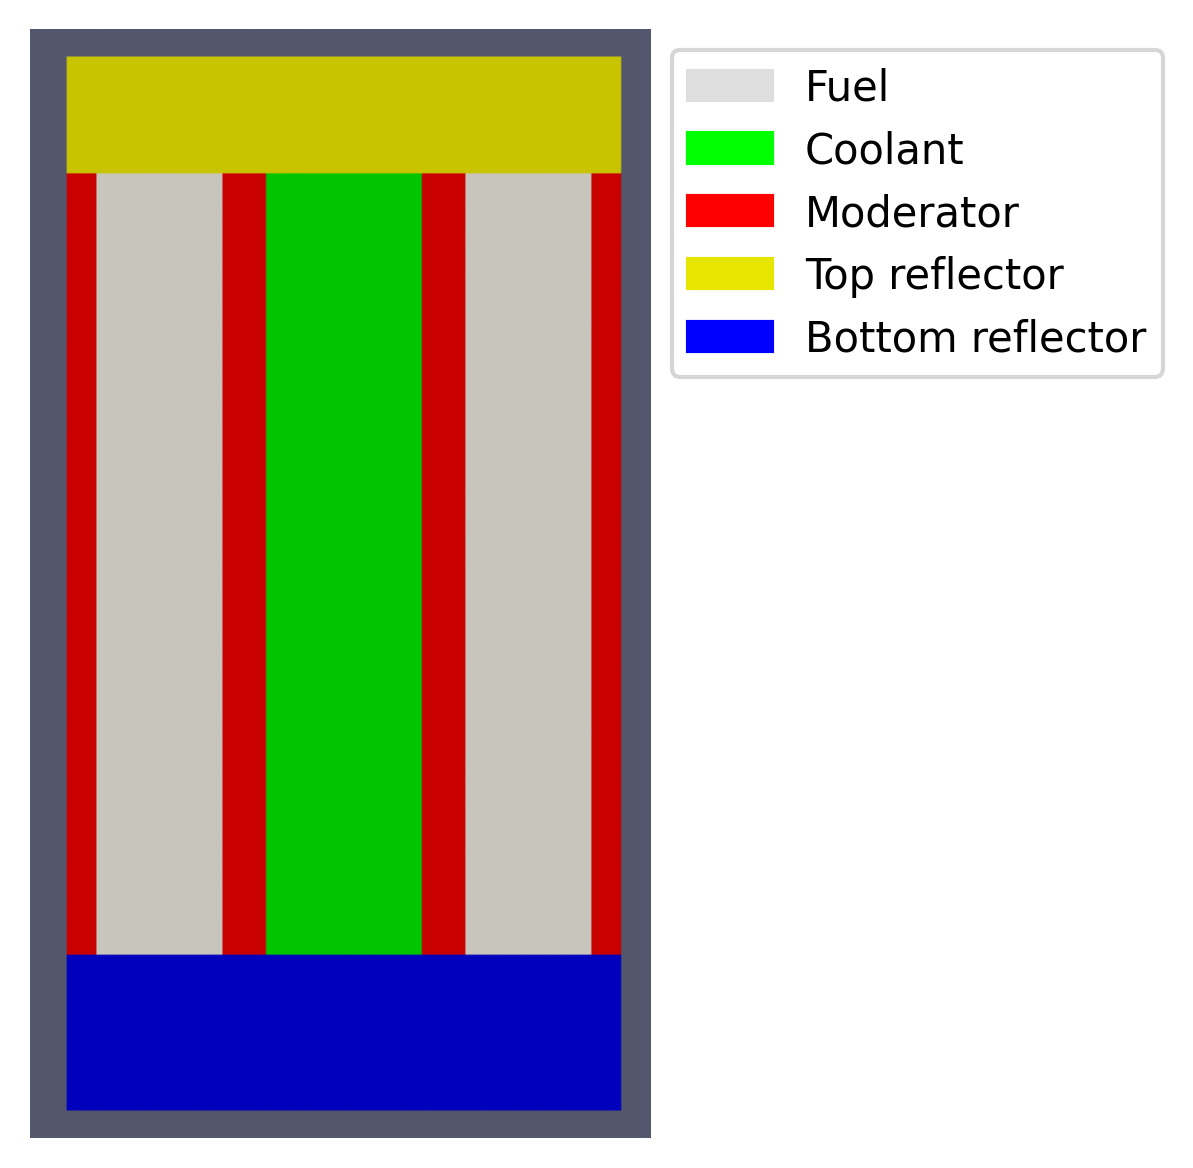
\includegraphics[height=5cm]{2D-unitcell-reflec-mesh}
		\caption{\textit{2D-unitcell-reflec} scaled down geometry.}
		\label{fig:2D-unitcell-reflec}
	\end{figure}

	\begin{figure}[htbp!]
		\centering
		\begin{subfigure}[t]{0.4\textwidth}
			\centering
			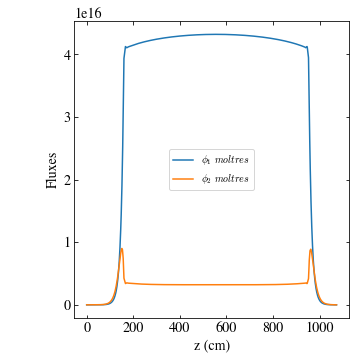
\includegraphics[width=\linewidth]{2D-unitcell-reflec-action1}
			\caption{Fuel centerline between points (0.94,-160,0) and (0.94,913,0).}
		\end{subfigure}
		\begin{subfigure}[t]{0.4\textwidth}
			\centering
			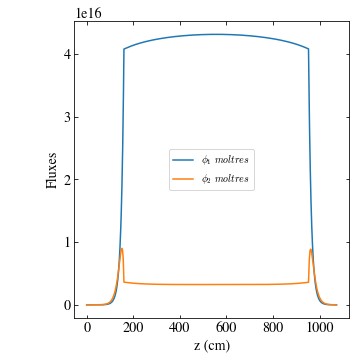
\includegraphics[width=\linewidth]{2D-unitcell-reflec-action2}
			\caption{Coolant centerline between points (2.82,-160,0) and (2.82,913,0).}
		\end{subfigure}
		\hfill
		\caption{Group 1 and 2 axial fluxes in different locations of the unitcell at 10 msec.}
		\label{fig:2D-unitcell-reflec1}
	\end{figure}

	\begin{figure}[htbp!]
		\centering
		\begin{subfigure}[t]{0.4\textwidth}
			\centering
			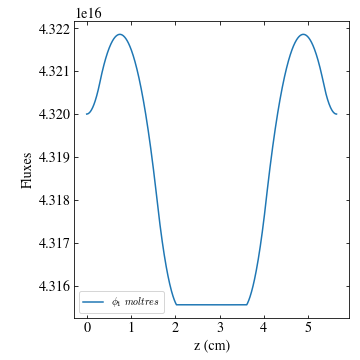
\includegraphics[width=\linewidth]{2D-unitcell-reflec-action3}
			\caption{Group 1.}
		\end{subfigure}
		\begin{subfigure}[t]{0.4\textwidth}
			\centering
			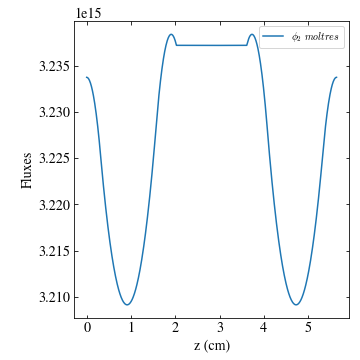
\includegraphics[width=\linewidth]{2D-unitcell-reflec-action4}
			\caption{Group 2.}
		\end{subfigure}
		\hfill
		\caption{Group 1 and 2 fluxes across the cell between points (0,400,0) and (5.64,400,0) at 10 msec.}
		\label{fig:2D-unitcell-reflec2}
	\end{figure}

\subsection{2D-fullcore-reflec-action}

	\begin{itemize}
		\item Input file: \textit{2D-fullcore-reflec-action.i}
		\item Mesh: \textit{2D-fullcore-reflec.msh}
		\item Transient problem.
	\end{itemize}

Figure \ref{fig:2D-fullcore-reflec} displays the geometry.
Figure \ref{fig:2D-unitcell-reflec2} shows the results.

	\begin{figure}[htbp!]
		\centering
		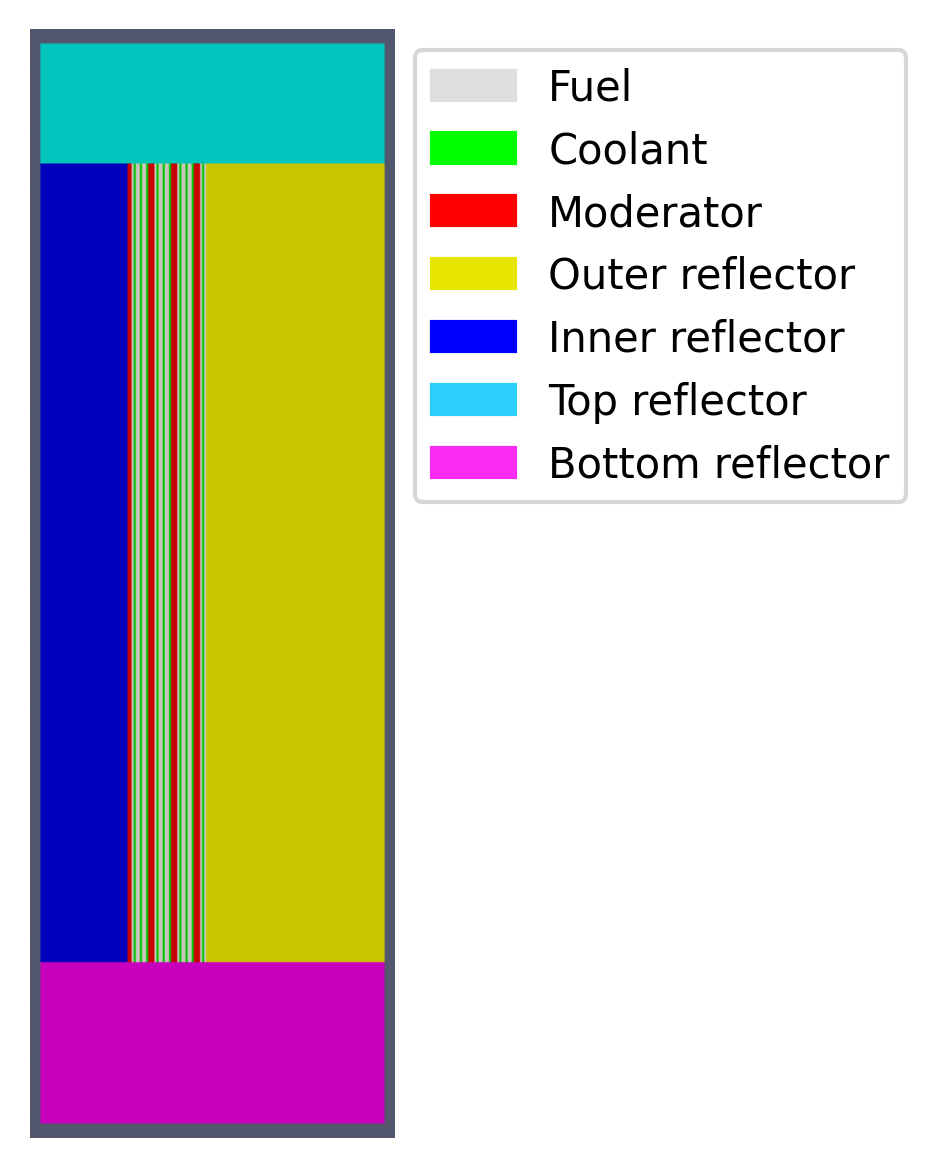
\includegraphics[height=8cm]{2D-fullcore-reflec-mesh}
		\caption{RZ-plane of \textit{2D-fullcore-reflec-action} geometry.}
		\label{fig:2D-fullcore-reflec}
	\end{figure}

	\begin{figure}[htbp!]
		\centering
		\begin{subfigure}[t]{0.4\textwidth}
			\centering
			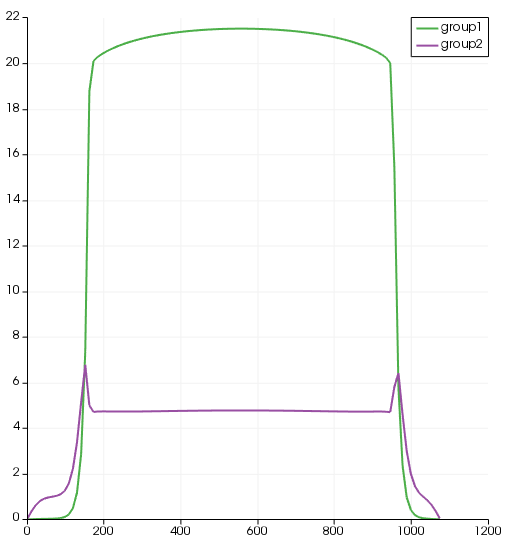
\includegraphics[width=\linewidth]{2D-fullcore-reflec-action1}
			\caption{Fuel centerline between points (162.94,-160,0) and (162.94,913,0).}
		\end{subfigure}
		\begin{subfigure}[t]{0.4\textwidth}
			\centering
			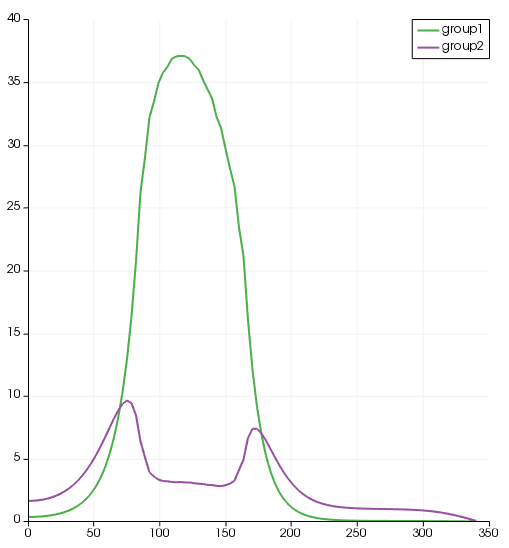
\includegraphics[width=\linewidth]{2D-fullcore-reflec-action2}
			\caption{Radial flux at y=400.}
		\end{subfigure}
		\hfill
		\caption{Group 1 and 2 fluxes at 1 msec.}
		\label{fig:2D-fullcore-reflec2}
	\end{figure}


\pagebreak
\bibliographystyle{plain}
% \bibliography{bibliography}

\end{document}
